%% TITLE	Physiological Fluid Mechanics, Summary 5

%% DATE		- May 17, 2022     first release
%%          - Nov 19, 2023      update

%% AUTHOR	BINGHUAN W LI (Dept. Chemical Eng/Bio Eng, Imperial)
%%          PETER Y XIE (Dept. Mech Eng, Stanford)

%% compiled in XeLaTeX with Tex Live version 2023.

%% This work is licensed under a Creative Commons Attribution-NonCommercial 4.0 International License.

\documentclass[a4paper]{article}
\newcommand{\summaryNo}{5}
%% TITLE	Physiological Fluid Mechanics, configuration

%% DATE		- Nov 19, 2023     create

%% AUTHOR	BINGHUAN W LI (Dept. Chemical Eng/Bio Eng, Imperial)
%%          PETER Y XIE (Dept. Mech Eng, Stanford)

%% compiled in XeLaTeX with Tex Live version 2023.

%% This work is licensed under a Creative Commons Attribution-NonCommercial 4.0 International License.

\usepackage[sfdefault]{arimo}
\usepackage[left=1.5cm, right=1.5cm, top=2cm, bottom=1.5cm]{geometry}
\usepackage{amsmath, amsfonts, amssymb, cancel}
\usepackage{unicode-math}
\setmathfont
    [    Extension = .otf,
         BoldFont = XITSMath-Bold,
    ]{XITSMath-Regular}

% % \DeclareMathSizes{10}{12}{10}{9}

% \usepackage{siunitx}
\usepackage{enumitem}
\usepackage{xcolor}
    \definecolor{linkcolour}{rgb}{0,0.2,0.6}
\usepackage{hyperref}
\hypersetup{
    colorlinks,
    breaklinks,
    urlcolor=linkcolour,
    linkcolor=linkcolour,
    citecolor=black,
    pdfauthor={Li, Binghuan W},
    }
\usepackage{graphicx, float}
\usepackage{framed}
\usepackage[export]{adjustbox}

\usepackage{fancyhdr}
    \pagestyle{fancy}
    \fancyhf{}
    \lhead{\textsc{Physiological Fluid Mechanics Summary \summaryNo}}
    \rhead{page \thepage}

\usepackage{tcolorbox}

\usepackage{tikz, circuitikz}

\usepackage{multicol}
    \setlength{\columnseprule}{1pt}

\usepackage{lscape}

\usepackage{booktabs}

\usepackage{pifont}

\setlength\parindent{0pt}

\begin{document}

% \begin{center}
%     \color{red} This is NOT an official formula booklet and will NOT be provided during your exam.
% \end{center}

\section{Finite Difference Method}
\paragraph{Governing equation}
\[
    \underbrace{\frac{\mathrm{d}^2 u}{\mathrm{d}x^2}}_{u''} + 2 \underbrace{\frac{\mathrm{d}u}{\mathrm{d}x}}_{u'} = 0
\]
\paragraph{Boundary conditions}
\begin{itemize}
    \item[-] $u=1$ at $x=0$,
    \item[-] $u=0$ at $x=1$.
\end{itemize}
\paragraph{Solution procedure}
With the Taylor series expansion
\begin{equation}
\label{eqn:prev_node}
    u(x_{i-1}) = u(x_i) - u'(x_i)\mathrm{d}x + \frac{1}{2}u''(x_i)\mathrm{d}x^2 - \frac{1}{6}u'''(x_i)\mathrm{d}x^3 + \mathcal{O}(\mathrm{d}x^4)
\end{equation}
\begin{equation}
\label{eqn:fwd_node}
    u(x_{i+1}) = u(x_i) + u'(x_i)\mathrm{d}x + \frac{1}{2}u''(x_i)\mathrm{d}x^2 + \frac{1}{6}u'''(x_i)\mathrm{d}x^3 + \mathcal{O}(\mathrm{d}x^4)
\end{equation}
Equation (\ref{eqn:prev_node}) + (\ref{eqn:fwd_node})
\begin{align*}
    u(x_{i-1}) + u(x_{i+1}) & = 2 u(x_i) + u''(x_i) \mathrm{d}x^2 + \mathcal{O}(\mathrm{d}x^4) \\
    & \Rightarrow {\color{red} u''(x_i) = \frac{1}{\mathrm{d}x^2} (u(x_{i-1}) - 2u(x_i) + u(x_{i+1})) + \mathcal{O}(\mathrm{d}x^2)}
\end{align*}

Equation (\ref{eqn:fwd_node}) - (\ref{eqn:prev_node})
\begin{align*}
    u(x_{i+1}) - u(x_{i-1}) & = 2 u'(x_i)\mathrm{d}x + \frac{1}{3}u'''(x_i) \mathrm{d}x^3 + \mathcal{O}(\mathrm{d}x^4) \\
    & \Rightarrow {\color{blue} u'(x_i) = \frac{1}{2\mathrm{d}x} (u(x_{i+1}) - u(x_{i-1})) + \mathcal{O}(\mathrm{d}x^2)}
\end{align*}
The methods shown above is commonly referred to as the \textbf{central differencing scheme}, which has a 2\textsuperscript{nd}-order accuracy.
Hence, the governing equation
\begin{align*}
    \Rightarrow \quad & {\color{red} \frac{1}{\mathrm{d}x^2} (u(x_{i-1}) - 2u(x_i) + u(x_{i+1})) + \cancel{\mathcal{O}(\mathrm{d}x^2)}} + {\color{blue} \frac{1}{\mathrm{d}x} (u(x_{i+1}) - u(x_{i-1})) + \cancel{\mathcal{O}(\mathrm{d}x^2)}} = 0 \\
    \Rightarrow \quad & \bigg(\frac{1}{\mathrm{d}x^2} - \frac{1}{\mathrm{d}x} \bigg) u_{i-1} + \bigg(-\frac{2}{\mathrm{d}x^2}\bigg)u_i + \bigg(\frac{1}{\mathrm{d}x^2}+\frac{1}{\mathrm{d}x}\bigg) u_{i+1} = 0
\end{align*}
For the index $i$ ranges from 1 to $N-1$, the above expression can be converted into the matrix form,
\[
    \underbrace{\begin{pmatrix}
        (-\frac{2}{\mathrm{d}x^2}) & (\frac{1}{\mathrm{d}x^2} + \frac{1}{\mathrm{d}x}) & 0 & 0 & \hdots & 0 & 0 \\
        (\frac{1}{\mathrm{d}x^2} - \frac{1}{\mathrm{d}x}) & (-\frac{2}{\mathrm{d}x^2}) & (\frac{1}{\mathrm{d}x^2} + \frac{1}{\mathrm{d}x}) & 0 & \hdots & 0 & 0 \\
        0 & (\frac{1}{\mathrm{d}x^2} - \frac{1}{\mathrm{d}x}) & (-\frac{2}{\mathrm{d}x^2}) & (\frac{1}{\mathrm{d}x^2} + \frac{1}{\mathrm{d}x}) & \hdots & 0 & 0 \\
        0 & 0 & (\frac{1}{\mathrm{d}x^2} - \frac{1}{\mathrm{d}x}) & (-\frac{2}{\mathrm{d}x^2}) & \hdots & 0 & 0 \\
        \vdots & \vdots & \vdots & \vdots & \ddots & 0 & 0 \\
        0 & 0 & 0 & 0 & \hdots & (-\frac{2}{\mathrm{d}x^2}) & (\frac{1}{\mathrm{d}x^2} + \frac{1}{\mathrm{d}x}) \\
        0 & 0 & 0 & 0 & \hdots & (\frac{1}{\mathrm{d}x^2} - \frac{1}{\mathrm{d}x}) & (-\frac{2}{\mathrm{d}x^2}) \\
    \end{pmatrix}}_{\mathbf{A}}
    \underbrace{\begin{pmatrix}
        u_1 \\
        u_2 \\
        u_3 \\
        u_4 \\
        \vdots \\
        u_{N-2} \\
        u_{N-1}
    \end{pmatrix}}_{\mathbf{u}}
    =
    \underbrace{\begin{pmatrix}
        -\frac{1}{\mathrm{d}x^2} + \frac{1}{\mathrm{d}x} \\
        0 \\
        0 \\
        0 \\
        \vdots \\
        0 \\
        0\\
    \end{pmatrix}}_{\mathbf{b}}
\]

\thispagestyle{empty}
\newgeometry{margin=1.8cm}
\mbox{}
\vfill    
\begin{figure}[H]
    \includegraphics[right]{images/by-nc.eps}
\end{figure}
\textit{This work is licensed under a Creative Commons Attribution-NonCommercial 4.0 International License.}


\end{document}